%%%%%%%%%%%%%%%%%%%%%%%%%%%%%%%%%%%%%%%%%%%%%%%%%%%%%%%%%%%
% --------------------------------------------------------
% Tau
% LaTeX Template
% Version 2.3.1 (10/04/2024)
%
% Author:
% Guillermo Jimenez (memo.notess1@gmail.com)
%
% License:
% Creative Commons CC BY 4.0
% --------------------------------------------------------
%%%%%%%%%%%%%%%%%%%%%%%%%%%%%%%%%%%%%%%%%%%%%%%%%%%%%%%%%%%
% --------------------------------------------------------
%     BIBLIOGRAPHY WITH BIBLATEX IN EXTERNAL EDITORS
% --------------------------------------------------------
% If the bibliography does not show up, try running the
% 'tau.cls' and 'tau.bib' file with biber from the
% MikTeX console or your preferred LaTeX distribution to
% generate the auxiliar files and (re)run the main.tex.
% --------------------------------------------------------
%%%%%%%%%%%%%%%%%%%%%%%%%%%%%%%%%%%%%%%%%%%%%%%%%%%%%%%%%%%
% --------------------------------------------------------
%					  FOR SPANISH BABEL
% --------------------------------------------------------
% \usepackage[spanish,es-nodecimaldot,es-noindentfirst]{babel}
% --------------------------------------------------------
%%%%%%%%%%%%%%%%%%%%%%%%%%%%%%%%%%%%%%%%%%%%%%%%%%%%%%%%%%%

\documentclass[9pt,a4paper,twoside]{tau}
\usepackage[english]{babel}
\usepackage{tauenvs}

%----------------------------------------------------------
% TITLE
%----------------------------------------------------------

\title{Título do relatório projeto final da disciplina de \textit{Reinforcement Learning}}

%----------------------------------------------------------
% AUTHORS, AFFILIATIONS AND PROFESSOR
%----------------------------------------------------------

\author[a]{Giancalo Vanoni Ruggiero}
\author[a]{Luciano Felix Dias}
\author[b]{Tales Ivalque}

%----------------------------------------------------------

\affil[a]{Engenharia da Computação, INSPER}
\affil[b]{Engenharia Mecatrônica, INSPER}

\professor{Prof. Fabrício Barth}

%----------------------------------------------------------
% FOOTER INFORMATION
%----------------------------------------------------------

\institution{INSPER}
\ftitle{}
\date{10 de maio de 2024}
\course{Reinforcement Learning}

%----------------------------------------------------------
% ABSTRACT
%----------------------------------------------------------

\begin{abstract}
    Neste projeto foi desenvolvido e validado um agente capaz de atuar no ambient XXX. O método de treinamento empregado foi ... Os resultados obtidos foram ...
\end{abstract}

%----------------------------------------------------------

\keywords{Reinforcement Learning, DQN, Taxi Driver, ...}

%----------------------------------------------------------

\begin{document}

\maketitle
\thispagestyle{firststyle}
\tauabstract
%	\tableofcontents

%----------------------------------------------------------

\section{Introdução}

\taustart{N}a introdução é importante apresentar o contexto e objetivo do trabalho. \textbf{Por que usar aprendizagem por reforço para resolver este problema?} Qual é otimização desejada?

\section{Ambiente}

Nesta seção é importante responder as seguintes perguntas:

\begin{itemize}
    \item \textbf{Como os estados são representados?} Não basta dizer que é um Box ou uma matriz RGB. É necessário explicar o motivo desta representação. Considerando o problema que pretende-se resolver, porque os autores do ambiente decidiram utilizar esta representação?
    \item \textbf{Qual é o espaço de ações do agente?} As ações são discretas ou contínuas? Se discretas, quantas são? O ambiente é determinístico ou não?
    \item \textbf{Como é definida a função de reward?}
\end{itemize}

Para responder algumas das perguntas acima, talvez seja necessário utilizar equações. Desta forma, segue alguns exemplo de como definirir equações em \LaTeX. Neste caso, são apresentados dois exemplos, a equação \ref{ec:equation} e a equação \ref{ec:equation2}.

\begin{equation} \label{ec:equation}
    \frac{\hbar^2}{2m}\nabla^2\Psi + V(\mathbf{r})\Psi = -i\hbar \frac{\partial\Psi}{\partial t}
\end{equation}

\begin{equation}\label{ec:equation2}
    f(x) = x^{2} +  2x + 10
\end{equation}


\section{Método}

Nesta seção é importante descrever os \textbf{algoritmos testados}. Uma breve descrição, não é necessário descrever detalhes do funcionamento do algoritmo. A equipe pode assumir que o leitor deste texto é alguém familiarizado com os algoritmos de reinforcement learning. Não esqueçam de colocar as \textbf{devidas citações}. Por exemplo:

\begin{info}[frametitle=Exemplo]
    Este artigo irá fazer uso dos algoritmos DQN \cite{mnih2013} e PPO \cite{schu2017} para treinar um agente para o ambiente XXX...
\end{info}

Também é importante destacar a implementação utilizada. Se foi uma implementação feita do zero pela equipe ou se foi utilizada uma biblioteca. Se a equipe optou por utilizar uma biblioteca é importante citar a biblioteca. Em ambos os casos, se a equipe fez a sua própria implementação ou se utilizou uma biblioteca, é importante \textbf{citar o repositório} onde os scripts se encontram.

Nesta seção também é importante descrever quais são os principais \textbf{indicadores} que a equipe está avaliando. Isto está diretamente relacionado com a função que pretende-se otimizar - que foi descrita na introdução deste relatório.

Eventualmente, a equipe deseja adicionar algum trecho de código nesta parte do relatório. Isto pode ser feito da seguinte maneira:

\lstinputlisting[caption=Exemplo de código em Python, language=python]{assets/example.py}

\section{Resultados}

O objetido desta pararte do relatório é descrever os resultados obtidos. Durante a disciplina nós vimos as principais técnicas para mostrar o aprendizado do agente e o desempenho do mesmo para realizar a tarefa. Esta seção precisa mostrar dados quantitativos que descrevem isto: a curva de aprendizagem e as validações feitas depois do treinamento.

Para apresentar os resultados obtidos com certeza a equipe terá que fazer uso de figuras, como a apresenta em \ref{fig:figure}.

\begin{figure}[htbp]
    \centering
    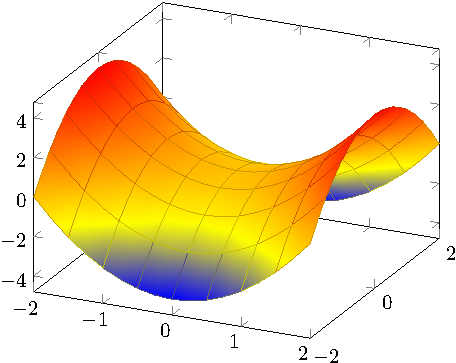
\includegraphics[width=0.8\columnwidth]{assets/example.pdf}
    \caption{Exemplo de figura obtido a partir de \textit{PGFPlots - A LaTeX package to create plots}. [Online]. Available: \url{https://pgfplots.sourceforge.net/}).}
    \label{fig:figure}
\end{figure}

Além de tabelas, como a apresentada em \ref{tab:table}.

\begin{table}[htbp]
    \caption{Exemplo de tabela}
    \label{tab:table}
    \centering
    \begin{tabular}{cc}
        \toprule
        \textbf{Column 1} & \textbf{Column 2} \\
        \midrule
        Data 1            & Data 2            \\
        Data 3            & Data 4            \\
        \bottomrule
    \end{tabular}
\end{table}

\section{Considerações finais}

\taustart{O} objetivo deste trabalho foi ...

\addcontentsline{toc}{section}{References}
\printbibliography

\end{document}
